\documentclass[11pt]{article}

\usepackage[T1]{fontenc}
\usepackage[utf8]{inputenc}
\usepackage{lmodern}
\usepackage[margin=0.85in]{geometry}
\usepackage{amsmath}
\usepackage{array}
\usepackage{booktabs}
\usepackage{graphicx}
\usepackage{hyperref}
\usepackage{tikz}
\usepackage{url}
\usetikzlibrary{arrows.meta,calc,fit,positioning,shapes.geometric}

\hypersetup{
  colorlinks=true,
  linkcolor=blue,
  citecolor=blue,
  urlcolor=blue
}

\newcommand{\filecutile}{\texttt{hpl\_ai/cutile\_hpl\_ai.py}}
\newcommand{\filedoc}{\texttt{cuTileGenDoc.md}}
\newcommand{\hplai}{HPL-AI}
\newcommand{\cutile}{cuTile}
\newcommand{\nixnan}{NixNan}
\newcommand{\code}[1]{\texttt{#1}}
\newcolumntype{P}[1]{>{\raggedright\arraybackslash}p{#1}}

\tikzset{
  flowbox/.style={draw, rounded corners=2pt, align=center, minimum height=0.78cm, text width=2.7cm, font=\small},
  wideflow/.style={draw, rounded corners=2pt, align=center, minimum height=0.88cm, text width=3.4cm, font=\small},
  hostbox/.style={flowbox, fill=gray!12},
  gpubox/.style={flowbox, fill=blue!8},
  decisionbox/.style={draw, diamond, aspect=2.1, align=center, inner sep=1pt, font=\small, fill=orange!12},
  arrow/.style={-{Latex[length=2mm]}, thick},
  lightarrow/.style={-{Latex[length=2mm]}, semithick},
  group/.style={draw, rounded corners=3pt, inner sep=6pt, dashed}
}

\title{HPL-AI to cuTile Porting Report\\
\large From the C Reference Path to Python and Quotient-Based GPU Kernels}
\author{cuTile analysis workspace}
\date{June 2026}

\begin{document}
\maketitle

\begin{abstract}
This report documents the local \hplai{} extraction in \filecutile{} as a
two-step port. The first step is an executable Python port of the compact C
reference path: matrix and right-hand-side generation, precision conversion,
no-pivot LU factorization, triangular solve, GMRES iterative refinement, and
the scaled residual check. The second step is a narrower \cutile{} port that
maps the dense, regular, low-level arithmetic kernels to GPU tile notation
while leaving generation, refinement, and validation on the host. The intent is
not to claim that every part of the benchmark has been made faster on the GPU.
The intent is to make the numerical decisions explicit, preserve the benchmark
semantics that matter for residual quality, and create compact kernels that are
good targets for \nixnan{} floating-point diagnostics.
\end{abstract}

\tableofcontents
\clearpage

\section{Purpose and Scope}

The local analysis directory already contains \filedoc{}, which is a
thorough, function-by-function note on the extraction. This document is a more
reader-oriented report intended to become a 12--14 page PDF. It starts from
\filecutile{}, treats the file as the central artifact, and records how the
program moves from an upstream C benchmark path to Python and then to \cutile{}
notation.

The upstream source identified by the existing notes is the Innovative
Computing Laboratory \hplai{} reference implementation
\cite{icl-hpl-ai}. \hplai{} itself sits in the same benchmark family as HPL,
the High Performance Linpack benchmark \cite{hpl-netlib}, but uses
mixed-precision linear algebra and iterative refinement to expose modern
accelerator arithmetic \cite{hpl-ai-top500}. The local file \filecutile{} is
therefore best read as a port of a specific benchmark path rather than as a
general linear-solver library.

Figure~\ref{fig:overall-flow} summarizes the end-to-end story. The important
division is that the Python port keeps the full algorithmic path executable,
while the \cutile{} port selects the GPU-sized arithmetic pieces that are
compact enough to inspect and diagnostic enough for \nixnan{}.

\begin{figure}[htbp]
\centering
\resizebox{\textwidth}{!}{%
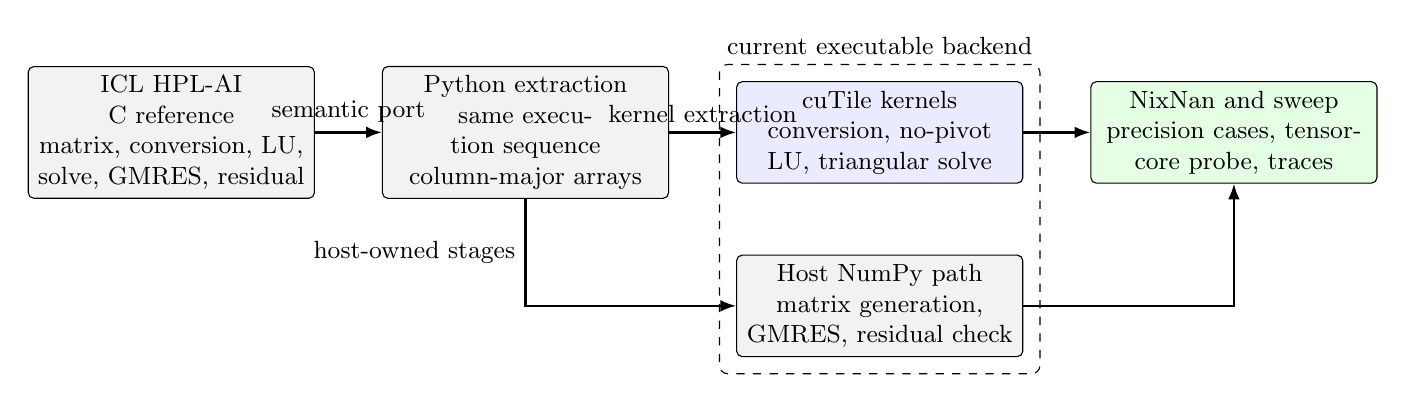
\begin{tikzpicture}[node distance=0.9cm and 0.85cm]
  \node[wideflow, fill=gray!10] (csrc) {ICL \hplai{} C reference\\matrix, conversion, LU, solve, GMRES, residual};
  \node[wideflow, fill=gray!10, right=of csrc] (py) {Python extraction\\same execution sequence\\column-major arrays};
  \node[wideflow, fill=blue!8, right=of py] (gpu) {\cutile{} kernels\\conversion, no-pivot LU, triangular solve};
  \node[wideflow, fill=gray!10, below=of gpu] (host) {Host NumPy path\\matrix generation, GMRES, residual check};
  \node[wideflow, fill=green!10, right=of gpu] (diag) {\nixnan{} and sweep\\precision cases, tensor-core probe, traces};

  \draw[arrow] (csrc) -- node[above, font=\small]{semantic port} (py);
  \draw[arrow] (py) -- node[above, font=\small]{kernel extraction} (gpu);
  \draw[arrow] (py) |- node[pos=0.25, left, font=\small]{host-owned stages} (host);
  \draw[arrow] (gpu) -- (diag);
  \draw[arrow] (host) -| (diag);

  \node[group, fit=(gpu)(host), label={[font=\small]above:current executable backend}] {};
\end{tikzpicture}}
\caption{End-to-end flow from the upstream C reference path to the local Python extraction, \cutile{} kernels, and diagnostic sweep artifacts.}
\label{fig:overall-flow}
\end{figure}

Two qualifications are useful at the start. First, the local port intentionally
keeps the HPL-style column-major storage model. This avoids hidden
transpositions when comparing the Python code, the \cutile{} kernels, and the C
reference. Second, the GPU mapping is selective. It is based on regularity,
data-parallel density, diagnostic value, and implementation risk. It is not a
blanket assertion that every operation in the full benchmark is better on a
GPU.

\section{Reading \filecutile{} as an HPL-AI Port}

The first evidence is explicit in the module docstring and the local license
file. \path{hpl_ai/cutile_hpl_ai.py} states that it is derived from the ICL \hplai{} reference
implementation and lists the extracted path:
generate the matrix and RHS, convert inputs, factor with no-pivot LU, solve the
triangular factors, convert the solution for refinement, optionally run GMRES,
and compute the scaled residual. The local \texttt{hpl\_ai/HPL\_AI\_LICENSE}
keeps the upstream license note.

The second evidence is structural. The Python functions are not independent
inventions with similar names. They mirror the reference benchmark's dataflow:
\code{hpl\_ai\_matrix} and \code{make\_rhs} cover the generator path,
\code{lu\_nopiv\_cpu} covers no-pivot LU, \code{lu\_solve\_cpu} covers the
forward and backward triangular solve, \code{gmres\_refine} covers
left-preconditioned refinement, and \code{scaled\_residual} covers the final
HPL-style acceptance metric.

\begin{figure}[htbp]
\centering
\resizebox{0.72\textwidth}{!}{%
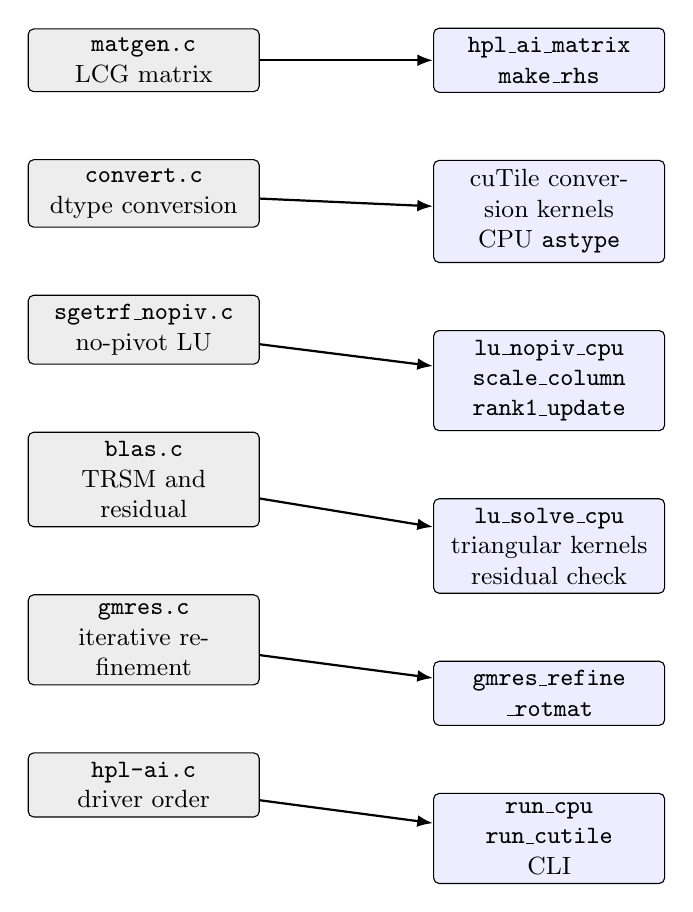
\begin{tikzpicture}[node distance=0.85cm and 0.85cm]
  \node[flowbox, fill=gray!14] (matgen) {\texttt{matgen.c}\\LCG matrix};
  \node[flowbox, fill=gray!14, below=of matgen] (convert) {\texttt{convert.c}\\dtype conversion};
  \node[flowbox, fill=gray!14, below=of convert] (getrf) {\texttt{sgetrf\_nopiv.c}\\no-pivot LU};
  \node[flowbox, fill=gray!14, below=of getrf] (blas) {\texttt{blas.c}\\TRSM and residual};
  \node[flowbox, fill=gray!14, below=of blas] (gmres) {\texttt{gmres.c}\\iterative refinement};
  \node[flowbox, fill=gray!14, below=of gmres] (driver) {\texttt{hpl-ai.c}\\driver order};

  \node[flowbox, fill=blue!7, right=2.2cm of matgen] (pymat) {\texttt{hpl\_ai\_matrix}\\\texttt{make\_rhs}};
  \node[flowbox, fill=blue!7, below=of pymat] (pyconv) {\cutile{} conversion kernels\\CPU \texttt{astype}};
  \node[flowbox, fill=blue!7, below=of pyconv] (pylu) {\texttt{lu\_nopiv\_cpu}\\\texttt{scale\_column}\\\texttt{rank1\_update}};
  \node[flowbox, fill=blue!7, below=of pylu] (pysolve) {\texttt{lu\_solve\_cpu}\\triangular kernels\\residual check};
  \node[flowbox, fill=blue!7, below=of pysolve] (pygmres) {\texttt{gmres\_refine}\\\texttt{\_rotmat}};
  \node[flowbox, fill=blue!7, below=of pygmres] (pydriver) {\texttt{run\_cpu}\\\texttt{run\_cutile}\\CLI};

  \foreach \a/\b in {matgen/pymat,convert/pyconv,getrf/pylu,blas/pysolve,gmres/pygmres,driver/pydriver}
    \draw[arrow] (\a) -- (\b);
\end{tikzpicture}}
\caption{Source-to-port correspondence used in the local notes. The port changes implementation form, but preserves the benchmark sequence.}
\label{fig:source-map}
\end{figure}

The C reference is compact, but it still carries several concerns at once:
storage layout, generator determinism, precision staging, factorization,
solve, refinement, and residual validation. The Python extraction deliberately
separates these concerns into small functions and dataclasses. This is the
first major design decision in the port. Instead of starting with the GPU, the
code first creates a host executable model whose behavior can be compared
against the \cutile{} backend.

The \code{PrecisionConfig} dataclass is central to that separation. The
reference benchmark has a mixed-precision intent, but the local analysis needs
to sweep multiple precision choices. The port therefore records five roles:
input precision, factorization precision, solve precision, refinement
precision, and residual precision. This keeps the benchmark default visible
while allowing the sweep to stress the low-precision stages.

The \code{MatrixConfig} dataclass is the analogous separation for matrix
generation. The upstream-like matrix kind is preserved as \code{hpl-ai}. A
second kind, \code{conditioned}, is added for controlled condition-number
experiments. This addition is explicitly not an upstream feature. It is an
analysis feature that lets the precision policy be studied under increasing
numerical stress.

\section{First Port: C Reference Algorithm to Python}

The first port converts the reference algorithm into readable Python while
preserving the algorithmic order and the memory indexing convention. It uses
NumPy arrays for the CPU oracle and records the exact flat column-major address
calculation:
\[
  \operatorname{index}(i,j,n) = i + jn.
\]
This is the Python form of the reference macro pattern that stores
\(A(i,j)\) at \code{row + col * lda}. Keeping that layout avoids a subtle
class of bugs. If the CPU path used row-major arrays and the \cutile{} path
used column-major buffers, comparing them would require additional layout
translations, and those translations could hide porting errors.

\begin{figure}[htbp]
\centering
\resizebox{\textwidth}{!}{%
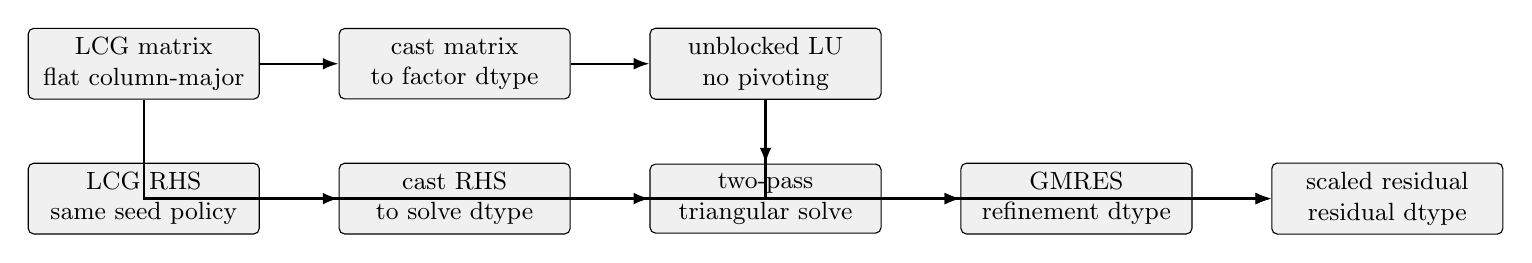
\begin{tikzpicture}[node distance=0.8cm and 1.0cm]
  \node[hostbox] (gena) {LCG matrix\\flat column-major};
  \node[hostbox, below=of gena] (genb) {LCG RHS\\same seed policy};
  \node[hostbox, right=of gena] (casta) {cast matrix\\to factor dtype};
  \node[hostbox, right=of genb] (castb) {cast RHS\\to solve dtype};
  \node[hostbox, right=of casta] (lu) {unblocked LU\\no pivoting};
  \node[hostbox, right=of castb] (solve) {two-pass\\triangular solve};
  \node[hostbox, right=of solve] (refine) {GMRES\\refinement dtype};
  \node[hostbox, right=of refine] (resid) {scaled residual\\residual dtype};

  \draw[arrow] (gena) -- (casta);
  \draw[arrow] (genb) -- (castb);
  \draw[arrow] (casta) -- (lu);
  \draw[arrow] (lu) -- (solve);
  \draw[arrow] (castb) -- (solve);
  \draw[arrow] (solve) -- (refine);
  \draw[arrow] (lu) |- (refine);
  \draw[arrow] (gena) |- (resid);
  \draw[arrow] (genb) |- (resid);
  \draw[arrow] (refine) -- (resid);
\end{tikzpicture}}
\caption{Python extraction data path. The host reference owns the full numerical sequence and is used as the executable oracle.}
\label{fig:python-path}
\end{figure}

\subsection{Matrix and RHS Generation}

The local generator is intentionally deterministic. The function
\code{\_lcg\_values} uses the same essential shape as the C generator: a
64-bit linear congruential generator, uint64 wraparound, and a scale factor
that produces values near the interval \([-0.5,0.5)\). The generated matrix is
then interpreted as an \(n \times n\) column-major matrix. The diagonal entries
are replaced by the sum of the off-diagonal absolute values in the same row.
The resulting matrix is row diagonally dominant, which is one of the reasons a
no-pivot LU path can be used as a benchmark path rather than as a general
purpose solver.

The right-hand side uses the same generator helper with a related seed. The
port keeps generation on the host because generation is not the diagnostic
target of this analysis. It also keeps the generator easy to compare with the
C reference. Moving the generator to a GPU kernel would add random-state and
layout surface area without improving the core question: whether the extracted
mixed-precision arithmetic kernels can be expressed compactly in \cutile{} and
observed by \nixnan{}.

\subsection{No-Pivot LU}

The upstream C reference uses no-pivot LU in a blocked or recursive style. The
Python extraction uses the mathematically equivalent unblocked outer-product
form:
\[
\begin{aligned}
  A_{k+1:n,k} &\leftarrow A_{k+1:n,k}/A_{k,k}, \\
  A_{k+1:n,k+1:n} &\leftarrow A_{k+1:n,k+1:n}
    - A_{k+1:n,k} A_{k,k+1:n}.
\end{aligned}
\]
This is a deliberate porting choice. The blocked schedule is better aligned
with high-performance GEMM use, but the unblocked form exposes the two
operations that need to become \cutile{} kernels: scale a pivot column and
apply a rank-1 update to the trailing matrix.

That choice trades some performance potential for clarity. In this local
analysis, clarity is valuable because the goal is to create a small GPU
surface that can be instrumented and reasoned about. The numerical operation
is still no-pivot LU. The scheduling strategy changed.

\subsection{Triangular Solve}

After factorization, the Python oracle performs a unit-lower forward solve and
a non-unit-upper backward solve. These loops are written in a way that mirrors
the future GPU mapping. Each pivot step updates a contiguous logical region of
the RHS vector. This makes it straightforward to compare the CPU version with
the \cutile{} kernels \code{forward\_subtract\_kernel},
\code{scale\_rhs\_kernel}, and \code{backward\_subtract\_kernel}.

The triangular solve remains lower intensity than the rank-1 trailing update,
but it is still mapped to \cutile{} because it is part of the extracted
mixed-precision solve path. If it remained only on the host, the \cutile{}
backend would no longer represent the complete low-precision factor-and-solve
phase. Keeping it on the GPU also avoids an unnecessary transfer between LU
factorization and the initial solution.

\subsection{GMRES and Residual}

The GMRES routine follows the standard generalized minimal residual structure
\cite{saad-schultz-gmres}: build Krylov vectors, orthogonalize, apply Givens
rotations, solve the small projected problem, and update the solution. In the
local code it is left-preconditioned by the LU factors. The residual check uses
the HPL-style scaled infinity-norm expression:
\[
  \frac{\|Ax-b\|_\infty}
  {\epsilon(\|A\|_\infty\|x\|_\infty+\|b\|_\infty)n}.
\]
The threshold is the local constant \code{RESIDUAL\_THRESHOLD = 16.0}.

Both GMRES and the residual check remain on the host in the current port. This
is not because they are unimportant. They are important to benchmark validity.
They stay on the host because they are not the smallest useful \cutile{}
surface. GMRES contains reductions, vector orthogonalization, small dense
solves, and control decisions. A high-quality GPU GMRES implementation would
require a separate design. The current report therefore treats host GMRES as
the validation and refinement layer around a GPU low-precision solve.

\section{Second Port: Python Extraction to cuTile}

The second port extracts the dense arithmetic operations from the Python model
and maps them to \cutile{} kernels. The resulting backend is
\code{run\_cutile}. It still generates matrix data on the host, but allocates
CuPy buffers, launches \cutile{} kernels for the factor-and-solve path, copies
the initial solution back, and optionally runs host GMRES.

\begin{figure}[htbp]
\centering
\resizebox{\textwidth}{!}{%
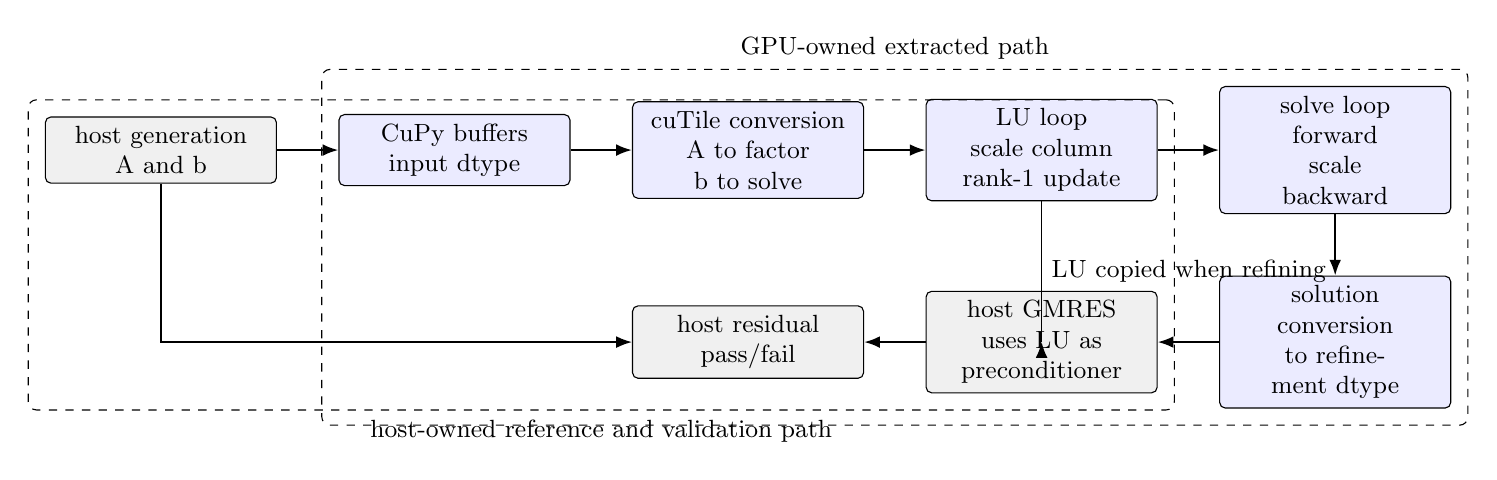
\begin{tikzpicture}[node distance=0.78cm and 0.78cm]
  \node[hostbox] (hostgen) {host generation\\A and b};
  \node[gpubox, right=of hostgen] (copy) {CuPy buffers\\input dtype};
  \node[gpubox, right=of copy] (conv) {\cutile{} conversion\\A to factor\\b to solve};
  \node[gpubox, right=of conv] (factor) {LU loop\\scale column\\rank-1 update};
  \node[gpubox, right=of factor] (trisolve) {solve loop\\forward\\scale\\backward};
  \node[gpubox, below=of trisolve] (xconv) {solution conversion\\to refinement dtype};
  \node[hostbox, left=of xconv] (hgmres) {host GMRES\\uses LU as preconditioner};
  \node[hostbox, left=of hgmres] (check) {host residual\\pass/fail};

  \draw[arrow] (hostgen) -- (copy);
  \draw[arrow] (copy) -- (conv);
  \draw[arrow] (conv) -- (factor);
  \draw[arrow] (factor) -- (trisolve);
  \draw[arrow] (trisolve) -- (xconv);
  \draw[arrow] (xconv) -- (hgmres);
  \draw[arrow] (hgmres) -- (check);
  \draw[lightarrow] (hostgen) |- (check);
  \draw[lightarrow] (factor) |- node[pos=0.25, right, font=\small]{LU copied when refining} (hgmres);

  \node[group, fit=(copy)(conv)(factor)(trisolve)(xconv), label={[font=\small]above:GPU-owned extracted path}] {};
  \node[group, fit=(hostgen)(hgmres)(check), label={[font=\small]below:host-owned reference and validation path}] {};
\end{tikzpicture}}
\caption{\cutile{} backend execution. The GPU owns conversion, no-pivot LU, and triangular solve; the host owns generation, refinement, and final validation.}
\label{fig:cutile-path}
\end{figure}

\subsection{Conversion Kernels}

The conversion kernels are intentionally simple. Each kernel loads a tile of
width \code{W=128}, casts it to the requested target dtype, masks inactive
lanes beyond the logical total, and stores the result. There are three
concrete kernels for \code{float16}, \code{float32}, and \code{float64}. The
helper \code{\_conversion\_kernel} chooses among them based on the precision
role currently being exercised.

Mapping conversion to \cutile{} is useful for two reasons. First, conversion is
part of the mixed-precision benchmark sequence. Second, it makes the precision
boundary explicit in the GPU trace. A run with \code{factor\_precision =
float16} and one with \code{factor\_precision = float32} do not merely change
a host dtype; they launch different conversion paths into GPU storage.

\subsection{LU Kernels}

The LU factorization becomes two kernels per pivot step. The first,
\code{scale\_column\_kernel}, divides each entry below the pivot by the pivot.
The second, \code{rank1\_update\_kernel}, updates the trailing matrix. The
rank-1 update is the largest regular arithmetic region in the unblocked LU
algorithm. It is therefore the clearest candidate for GPU mapping.

This mapping also makes an important performance distinction. The port does
not currently use tensor-core GEMM for the LU update. The rank-1 update is
scalar tile code. The separate tensor-core probe in the sweep exists to force
WMMA SASS for \nixnan{} verification, not to claim that the LU update itself
is tensor-core optimized. That distinction matters for interpreting traces.

\subsection{Triangular-Solve Kernels}

The triangular solve becomes a sequence of vector update kernels. Forward
substitution updates rows below the pivot. Backward substitution first scales
the pivot entry and then updates rows above the pivot. These operations are
less parallel than a full trailing matrix update because each pivot step
depends on the previous pivot result. Still, within each step the row updates
are independent, and the solve belongs to the same low-precision phase as the
factorization.

\subsection{Launch Structure}

The \cutile{} driver uses \code{\_grid\_for(total)} to compute a one-dimensional
tile grid. A logical element id is computed from the block id and lane id:
\[
  \operatorname{flat} = \operatorname{bid}_0 W + \operatorname{lane}.
\]
Kernels use masks so extra lanes in the last tile do not write outside the
logical region. This makes each kernel shape independent from exact matrix
sizes. The same tile width can cover an entire matrix buffer, a trailing
submatrix, or a vector segment.

\section{Quotient-Based Iteration Mapping}

The phrase quotient-based implementation is most concrete in the
\code{rank1\_update\_kernel}. A two-dimensional trailing matrix is represented
as one flat iteration space. Each active lane computes a flat id, then uses
quotient and remainder operations to recover the logical row and column:
\[
\begin{aligned}
  q &= \left\lfloor \frac{\operatorname{flat}}{\operatorname{trailing}} \right\rfloor, \\
  r &= \operatorname{flat} \bmod \operatorname{trailing}, \\
  \operatorname{row} &= k + 1 + r, \\
  \operatorname{col} &= k + 1 + q.
\end{aligned}
\]
The final matrix address is still column-major:
\[
  \operatorname{index} = \operatorname{row} + \operatorname{col} n.
\]

\begin{figure}[htbp]
\centering
\resizebox{0.95\textwidth}{!}{%
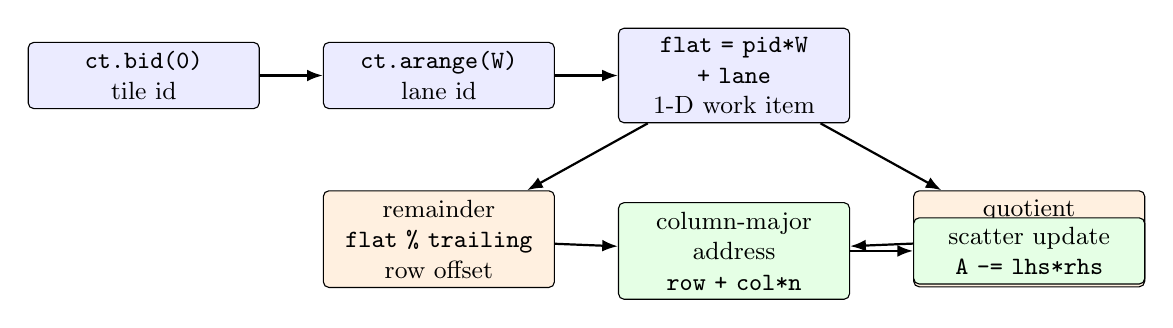
\begin{tikzpicture}[node distance=0.85cm and 0.8cm]
  \node[flowbox, fill=blue!8] (pid) {\texttt{ct.bid(0)}\\tile id};
  \node[flowbox, fill=blue!8, right=of pid] (lane) {\texttt{ct.arange(W)}\\lane id};
  \node[flowbox, fill=blue!8, right=of lane] (flat) {\texttt{flat = pid*W + lane}\\1-D work item};
  \node[flowbox, fill=orange!12, below left=of flat] (rem) {remainder\\\texttt{flat \% trailing}\\row offset};
  \node[flowbox, fill=orange!12, below right=of flat] (quo) {quotient\\\texttt{flat // trailing}\\column offset};
  \node[flowbox, fill=green!10, below=1.0cm of flat] (addr) {column-major address\\\texttt{row + col*n}};
  \node[flowbox, fill=green!10, right=of addr] (update) {scatter update\\\texttt{A -= lhs*rhs}};

  \draw[arrow] (pid) -- (lane);
  \draw[arrow] (lane) -- (flat);
  \draw[arrow] (flat) -- (rem);
  \draw[arrow] (flat) -- (quo);
  \draw[arrow] (rem) -- (addr);
  \draw[arrow] (quo) -- (addr);
  \draw[arrow] (addr) -- (update);
\end{tikzpicture}}
\caption{Quotient and remainder decomposition used to map a flat tile-lane iteration space back to trailing-matrix coordinates.}
\label{fig:quotient-map}
\end{figure}

This quotient-based form has several advantages for the current port.
First, it gives the kernel one simple grid dimension. The driver does not need
to create a two-dimensional launch for a submatrix whose size shrinks every
pivot. Second, it makes the logical operation easy to audit. Every active lane
performs the same algebraic update:
\[
  A_{\operatorname{row},\operatorname{col}}
  \leftarrow
  A_{\operatorname{row},\operatorname{col}}
  - A_{\operatorname{row},k} A_{k,\operatorname{col}}.
\]
Third, it naturally preserves the column-major memory layout. The quotient
identifies the column offset, the remainder identifies the row offset, and the
final address is the same expression used by the CPU oracle.

The tradeoff is that the mapping is not a tuned GEMM schedule. It is a clear
rank-1 update schedule. A high-performance implementation would likely block
the update, improve memory reuse, and use matrix-multiply primitives where
appropriate. The current quotient-based implementation is therefore best
understood as a faithful, inspectable mapping of the unblocked algorithm rather
than as a final performance implementation.

\section{Host/GPU Boundary and Rationale}

The boundary between host and GPU is the main engineering choice in the port.
Figure~\ref{fig:boundary} and Table~\ref{tab:boundary} summarize the decision.
The GPU receives the regular factor-and-solve arithmetic. The host retains
generation, conditioning experiments, GMRES refinement, and residual checking.

\begin{figure}[htbp]
\centering
\resizebox{\textwidth}{!}{%
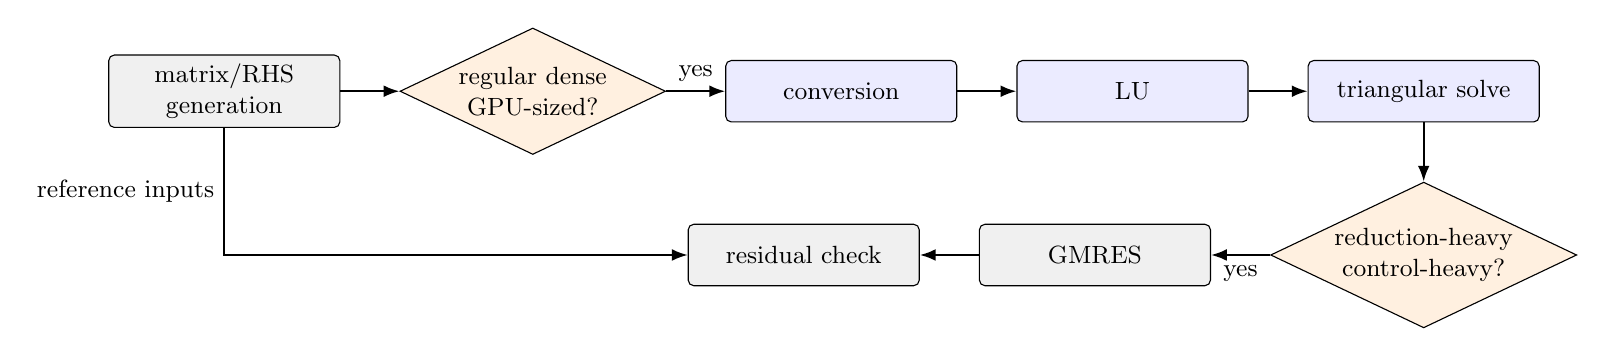
\begin{tikzpicture}[node distance=0.75cm and 0.75cm]
  \node[hostbox] (mg) {matrix/RHS\\generation};
  \node[decisionbox, right=of mg] (d1) {regular dense\\GPU-sized?};
  \node[gpubox, right=of d1] (conv) {conversion};
  \node[gpubox, right=of conv] (lu) {LU};
  \node[gpubox, right=of lu] (tr) {triangular solve};
  \node[decisionbox, below=of tr] (d2) {reduction-heavy\\control-heavy?};
  \node[hostbox, left=of d2] (gm) {GMRES};
  \node[hostbox, left=of gm] (rs) {residual check};

  \draw[arrow] (mg) -- (d1);
  \draw[arrow] (d1) -- node[above, font=\small]{yes} (conv);
  \draw[arrow] (conv) -- (lu);
  \draw[arrow] (lu) -- (tr);
  \draw[arrow] (tr) -- (d2);
  \draw[arrow] (d2) -- node[below, font=\small]{yes} (gm);
  \draw[arrow] (gm) -- (rs);
  \draw[lightarrow] (mg) |- node[pos=0.25, left, font=\small]{reference inputs} (rs);
\end{tikzpicture}}
\caption{Boundary decision used by the current port. The decision is based on regularity, diagnostic value, and implementation risk.}
\label{fig:boundary}
\end{figure}

\begin{table}[htbp]
\centering
\small
\begin{tabular}{P{0.24\textwidth}P{0.16\textwidth}P{0.52\textwidth}}
\toprule
Stage & Location & Rationale \\
\midrule
LCG matrix and RHS generation & Host & Determinism and reference comparability matter more than GPU throughput. Moving it would add state-management surface with little diagnostic value. \\
Conditioned matrix construction & Host & QR factorization and eigenvalue-spectrum construction are analysis scaffolding, not upstream benchmark work. \\
Precision conversion & GPU & Conversion is part of the mixed-precision path and creates visible GPU dtype boundaries. \\
No-pivot LU factorization & GPU & The scale and rank-1 update steps are regular dense arithmetic and are the best compact \cutile{} workload seed. \\
Triangular solve & GPU & It completes the low-precision factor-and-solve phase and avoids transferring intermediate LU/RHS state back to the host. \\
GMRES refinement & Host & Orthogonalization, reductions, small solves, and convergence checks make this a larger GPU project. Host execution preserves benchmark semantics while keeping the \cutile{} surface compact. \\
Scaled residual & Host & Validation needs high precision, stable norms, and simple comparability with the CPU oracle. \\
\bottomrule
\end{tabular}
\caption{Host/GPU placement decisions in the current extraction.}
\label{tab:boundary}
\end{table}

The boundary was not chosen only by asking which parts might run faster on a
GPU. Speedup potential matters, but it is only one criterion. The chosen GPU
parts are also the parts that can be expressed without a large runtime
protocol: each lane owns one matrix or vector element update, the active set is
controlled by a mask, and the kernels expose the floating-point operations that
\nixnan{} is meant to observe.

The host parts are retained because their role is different. Matrix generation
defines reproducible input. The conditioned matrix path defines a numerical
stress axis. GMRES protects the mixed-precision solve by applying a
higher-precision correction. The residual check is the benchmark acceptance
test. These stages can be GPU accelerated in a larger project, but mapping
them first would make the port harder to validate.

\section{Precision Choices as an Engineering Contract}

The default precision configuration in \filecutile{} is:
\begin{align*}
\text{input} &= \texttt{float64}, &
\text{factor} &= \texttt{float32}, &
\text{solve} &= \texttt{float32}, \\
\text{refinement} &= \texttt{float64}, &
\text{residual} &= \texttt{float64}.
\end{align*}
This is HPL-AI-like: use lower precision for the expensive factor-and-solve
phase, then use higher precision for iterative refinement and validation. The
choice reflects the standard mixed-precision idea that a low-precision solve
can be a preconditioner for a high-precision correction, provided the problem
and the low-precision factorization are stable enough \cite{higham-accuracy}.

\begin{figure}[htbp]
\centering
\resizebox{\textwidth}{!}{%
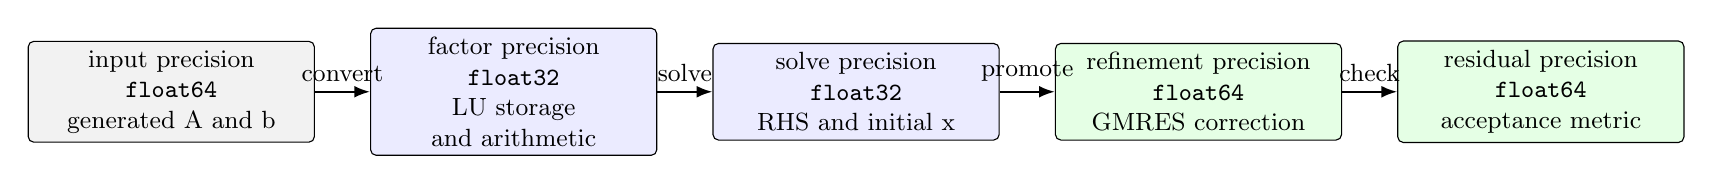
\begin{tikzpicture}[node distance=0.78cm and 0.7cm]
  \node[wideflow, fill=gray!10] (in) {input precision\\\texttt{float64}\\generated A and b};
  \node[wideflow, fill=blue!8, right=of in] (fac) {factor precision\\\texttt{float32}\\LU storage and arithmetic};
  \node[wideflow, fill=blue!8, right=of fac] (sol) {solve precision\\\texttt{float32}\\RHS and initial x};
  \node[wideflow, fill=green!10, right=of sol] (ref) {refinement precision\\\texttt{float64}\\GMRES correction};
  \node[wideflow, fill=green!10, right=of ref] (res) {residual precision\\\texttt{float64}\\acceptance metric};

  \draw[arrow] (in) -- node[above, font=\small]{convert} (fac);
  \draw[arrow] (fac) -- node[above, font=\small]{solve} (sol);
  \draw[arrow] (sol) -- node[above, font=\small]{promote} (ref);
  \draw[arrow] (ref) -- node[above, font=\small]{check} (res);
\end{tikzpicture}}
\caption{Precision pipeline used by the default configuration. The low-precision phase is bounded by high-precision refinement and residual validation.}
\label{fig:precision-pipeline}
\end{figure}

\subsection{Input Precision}

The default input precision is \code{float64}. This gives the generated system
a high-precision reference representation before any deliberate low-precision
conversion. It also makes residual checks meaningful: the final validation can
compare against the same high-precision input used by the CPU oracle.

When input precision is reduced, the experiment changes. The solver is no
longer only testing low-precision factorization and solve; it is also testing
whether the problem itself has been quantized. That is useful for stress
studies, but it is a different question from the HPL-AI-like default.

\subsection{Factor and Solve Precision}

The factorization and triangular solve default to \code{float32}. This is the
core mixed-precision compromise. It is low enough to expose accelerator-style
arithmetic and higher throughput than double precision on many GPUs, while
remaining much less fragile than \code{float16} for no-pivot LU.

The code allows \code{float16} factor and solve precision because the sweep is
designed to expose exceptional values and precision stress. However,
\code{float16} is not treated as the safe default for the LU path. No-pivot LU
can amplify rounding and pivot-growth effects. With a difficult matrix,
\code{float16} may overflow, underflow, or produce a singular effective
factorization. Those failures are not surprising; they are useful diagnostic
cases.

\subsection{Refinement and Residual Precision}

GMRES refinement and residual checking default to \code{float64}. This is the
guardrail around the low-precision solve. The initial low-precision solution is
not accepted by construction. It must be corrected and then pass the scaled
residual threshold. Keeping this work in double precision reduces the chance
that the validation logic hides the same rounding effects that the experiment
is trying to study.

The residual precision is especially important. If the residual were computed
in the same low precision as the factorization, a poor solve could appear less
poor because the residual computation itself lost information. The local
default therefore separates solve speed from validation quality.

\section{Precision Policy as Condition Number Increases}

Condition number changes the precision story because forward error is
amplified by the sensitivity of the linear system. A rough rule is that
rounding effects scale with a factor like \(\kappa(A)u\), where \(u\) is the
unit roundoff of the relevant arithmetic \cite{higham-accuracy}. This rule is
not a complete stability guarantee for no-pivot LU, but it explains why the
same precision configuration can work on a benign matrix and fail on a more
ill-conditioned one.

\begin{figure}[htbp]
\centering
\resizebox{\textwidth}{!}{%
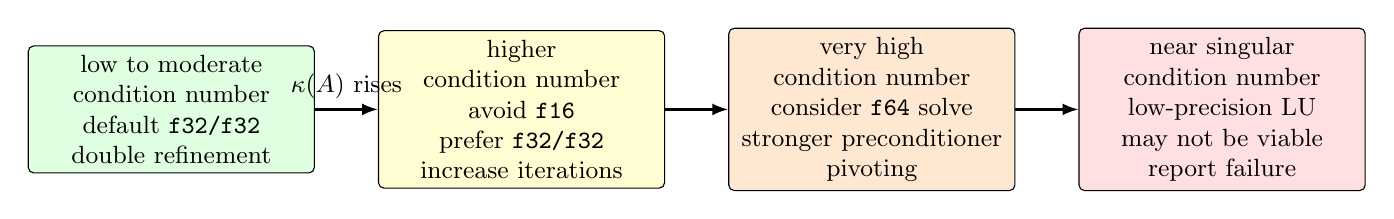
\begin{tikzpicture}[node distance=0.85cm and 0.8cm]
  \node[wideflow, fill=green!12] (low) {low to moderate\\condition number\\default \texttt{f32/f32}\\double refinement};
  \node[wideflow, fill=yellow!18, right=of low] (mid) {higher\\condition number\\avoid \texttt{f16}\\prefer \texttt{f32/f32}\\increase iterations};
  \node[wideflow, fill=orange!18, right=of mid] (high) {very high\\condition number\\consider \texttt{f64} solve\\stronger preconditioner\\pivoting};
  \node[wideflow, fill=red!12, right=of high] (extreme) {near singular\\condition number\\low-precision LU may not be viable\\report failure};

  \draw[arrow] (low) -- node[above, font=\small]{\(\kappa(A)\) rises} (mid);
  \draw[arrow] (mid) -- (high);
  \draw[arrow] (high) -- (extreme);
\end{tikzpicture}}
\caption{Qualitative precision ladder as condition number rises. The exact cutoff is problem-dependent; the direction of the policy is the important point.}
\label{fig:condition-ladder}
\end{figure}

Table~\ref{tab:condition-policy} gives a practical policy for the local
experiments. The bands are intentionally qualitative. They should be read as
engineering guidance for sweeps, not as mathematical guarantees.

\begin{table}[htbp]
\centering
\small
\setlength{\tabcolsep}{4pt}
\begin{tabular}{P{0.18\textwidth}P{0.20\textwidth}P{0.20\textwidth}P{0.33\textwidth}}
\toprule
Condition regime & Factor/solve choice & Refinement/residual & Reasoning \\
\midrule
Benign or moderate & \code{float32}/\code{float32}; \code{float16} may be used as a stress case & \code{float64}/\code{float64} & The low-precision solve is likely to be a usable preconditioner, and double refinement can correct remaining error. \\
Rising condition number & Prefer \code{float32}/\code{float32}; avoid \code{float16} as a production setting & Keep \code{float64}/\code{float64}; allow more GMRES iterations & Sensitivity starts to magnify low-precision factorization error. Refinement needs a stronger initial solve. \\
High condition number & Consider \code{float64} solve precision or \code{float64} factorization for comparison & Keep \code{float64}; inspect convergence and residual history & The low-precision LU factor may no longer be a reliable preconditioner. Higher precision becomes diagnostic, not just conservative. \\
Near singular or unstable no-pivot case & Low-precision no-pivot LU should be expected to fail & Double residual should report failure clearly & The current algorithm lacks pivoting. A robust solver would need pivoting, equilibration, or a different preconditioner. \\
\bottomrule
\end{tabular}
\caption{Suggested precision policy for condition-number sweeps in this workspace.}
\label{tab:condition-policy}
\end{table}

The most important adjustment is to promote the factor-and-solve phase before
weakening validation. If the condition number goes up, the residual precision
should not be reduced to make the result pass. Instead, the low-precision
phase should become more accurate, or the algorithm should admit that the
chosen no-pivot factorization is not adequate for that matrix.

This is also why the \code{conditioned} matrix family is useful. The upstream
\hplai{} matrix generator does not expose a condition-number parameter. The
local conditioned family creates a controlled axis for experiments:
same backend, same precision roles, but increasing numerical sensitivity.
That makes it possible to distinguish implementation bugs from expected
precision breakdown.

\section{Verification and Diagnostic Use}

The local workflow has three layers of verification. First, the CPU path can
run without CUDA and validates the Python extraction. Second, the \cutile{}
backend can be compared against the CPU path with \code{--compare-cpu}. Third,
the \nixnan{} sweep can collect floating-point diagnostic traces around the
GPU work.

\begin{figure}[htbp]
\centering
\resizebox{0.95\textwidth}{!}{%
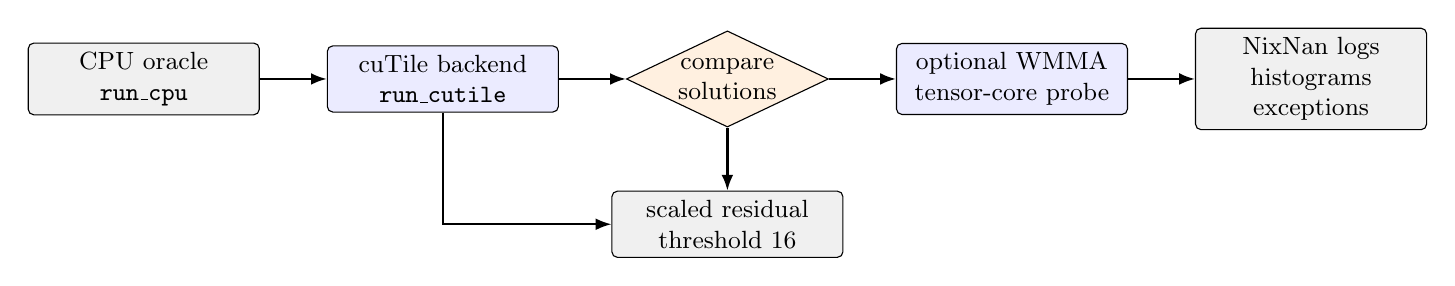
\begin{tikzpicture}[node distance=0.8cm and 0.85cm]
  \node[hostbox] (cpu) {CPU oracle\\\texttt{run\_cpu}};
  \node[gpubox, right=of cpu] (gpu) {\cutile{} backend\\\texttt{run\_cutile}};
  \node[decisionbox, right=of gpu] (cmp) {compare\\solutions};
  \node[hostbox, below=of cmp] (res) {scaled residual\\threshold 16};
  \node[gpubox, right=of cmp] (probe) {optional WMMA\\tensor-core probe};
  \node[hostbox, right=of probe] (trace) {\nixnan{} logs\\histograms\\exceptions};

  \draw[arrow] (cpu) -- (gpu);
  \draw[arrow] (gpu) -- (cmp);
  \draw[arrow] (cmp) -- (probe);
  \draw[arrow] (cmp) -- (res);
  \draw[arrow] (probe) -- (trace);
  \draw[lightarrow] (gpu) |- (res);
\end{tikzpicture}}
\caption{Verification and diagnostic layers used by the local sweep scripts.}
\label{fig:verification}
\end{figure}

The tensor-core probe deserves explicit separation. It is a small
FP16-by-FP16 to FP32 WMMA kernel, implemented through CuPy raw CUDA code and
using the CUDA WMMA interface \cite{nvidia-cuda-guide}. It exists so that the
\nixnan{} run can confirm HMMA instruction instrumentation. It is not the
implementation of the \cutile{} LU update. This separation is healthy: the
trace can include tensor-core evidence without overstating what the solver
kernels themselves do.

The sweep scripts record stdout, \nixnan{} logs, run environment, and a summary
table. They also expose the precision tuple:
\[
  (\text{input}, \text{factor}, \text{solve}, \text{refinement}, \text{residual}).
\]
That tuple is the practical interface between the numerical policy described
above and the diagnostic traces collected below it.

\section{Limitations and Next Iterations}

The current port is intentionally conservative. It provides a readable and
diagnostic extraction, not a final high-performance benchmark replacement.
The main limitations are as follows.

\begin{itemize}
  \item The LU implementation is unblocked. This makes the \cutile{} kernels
  small and inspectable, but it leaves performance on the table compared with
  blocked GEMM-based schedules.
  \item The factorization is no-pivot. This matches the extracted benchmark
  path, but it is not a robust general solver for arbitrary matrices.
  \item GMRES remains on the host. A GPU GMRES port would need careful design
  for reductions, orthogonalization, and small projected solves.
  \item The conditioned matrix family is an analysis extension. It should not
  be confused with the upstream generator.
  \item The tensor-core probe is separate from the solver. It verifies
  instrumentation coverage for HMMA instructions, not tensor-core acceleration
  of the LU path.
\end{itemize}

The next useful LaTeX iteration would add line-numbered code excerpts from
\path{hpl_ai/cutile_hpl_ai.py}, a short derivation of the scaled residual, and
a table of actual sweep cases from \path{nixnan_sweep/data/summary.tsv}.
Another useful iteration would compare the unblocked quotient-based update
with a hypothetical blocked update, making clear what would need to change
before pursuing performance rather than diagnostic clarity.

\section{Conclusion}

\filecutile{} is a port of the compact \hplai{} reference path into a Python
executable model and then into a selective \cutile{} backend. The first port
preserves benchmark semantics: deterministic generation, column-major layout,
mixed-precision no-pivot LU, triangular solve, GMRES refinement, and scaled
residual validation. The second port maps the dense low-level arithmetic into
tile kernels: conversion, column scaling, rank-1 trailing update, and
triangular-solve updates.

The host/GPU split is a deliberate boundary. GPU kernels are chosen where the
work is regular, dense, compact, and diagnostically valuable. Host execution is
kept where reference comparability, refinement correctness, and residual
validation matter more than a first-pass GPU speedup. The default precision
policy follows the mixed-precision benchmark idea: low precision for the
factor-and-solve phase, double precision for correction and validation. As
condition number rises, the policy should strengthen the low-precision phase
or report failure, not weaken the residual check.

\bibliographystyle{plain}
\bibliography{cutile_hpl_ai_porting_report}

\end{document}
